\section{Diskussion der Ergebnisse}
\label{sec:diskussion}
%7.) Inhalt des Kapitels: „Diskussion der Ergebnisse
%- Die Ergebnisse des Versuches und der in der Versuchsanleitung geforde
%Bestimmung einzelner Parameter soll unter wissenschaftlichen Aspekten disku
%werden. Dazu ist u.a. folgenden Fragen nachzugehen: Was sagen die Ergebn
%aus? Welche Annahmen und Näherungen wurden für die Ergebnisfindung gema
%Sind die Ergebnisse plausibel und decken sich mit Literatur- bzw. ande
%Vergleichswerten? Was sind mögliche Fehlerquellen und wie groß wird ihr Einf
%abgeschätzt?
%- Vergleich und Einordnung der eigenen Ergebnisse zu Literaturwerten
%- Abschluss des Kapitels: Finale Wertung der erarbeiteten Ergebnisse und Darstellung
%ihrer Kernaussage in kurzer prägnanter Form.
\begin{enumerate}[a)]
	\item \textit{Eine Gas- und eine Flüssigkeitsphase eines Einstoffsystems stehen während des Verdampfens und der Verflüssigung miteinander im Gleichgewicht. Wie werden der dazugehörige Druck und die dazugehörige Temperatur bezeichnet?}
	
	Die dazugehörige Temperatur wird kritische Temperatur $T_k$ genannt und der dazugehörige Druck beschreibt den kritischen Druck $p_k$.
	
	\item  \textit{Welche Einheit hat der Virialkoeffizient in den Gleichungen 3a und 3b? Und welche Form der Virialgleichung ist noch gebräuchlich in der Anwendung?}	
	\begin{flalign}
		p[\si{\bar}]*V[\si{\raiseto{3} \meter}] &= n[\si{\mol}]*R\left[\si{\joule \per \mol\per \kelvin}\right]*T[\si{\kelvin}]+n[\si{\mol}]*B(T)\left[\si{\raiseto{3}\meter \per\mol}\right]*p[\si{\bar}] \nonumber
	\end{flalign}
	Ebenfalls gebräuchliche Form der Virialgleichung: Leiden-Form
	\begin{flalign}
		p*V_m=R*T*\left(1+\frac{B}{V_m}+\frac{C}{V_m^2}+\frac{D}{V_m^3}+...\right)\nonumber
	\end{flalign}
	
	\item \textit{Stellen Sie dar, warum die Van-der-Waals-Gleichung den kubischen Zustandsgleichungen zugeordnet wird.}
	\begin{flalign}
		\tag{ausmultiplizieren}
		\left(p+\frac{a}{{V_m}^2}\right)*\left(V_m-b\right) &= R*T\\ \tag{$*{V_m}^2$}
		p*V_m-p*b+\frac{a}{V_m}-\frac{a*b}{{V_m}^2}	&= R*T\\		\tag{$:p$}
		p*{V_m}^3-p*b*{V_m}^2+a*V_m-a*b-R*T*{V_m}^2 &= 0\\	
		\mathbf{{V_m}^3-\left(b+\frac{R*T}{p}\right){V_m}^2+\frac{a}{p}*V_m-\frac{a*b}{p} }&\mathbf{=0}
	\end{flalign}
	
	\item 	\textit{Was ist unter dem kritischen Punkt und was unter dem Tripelpunkt eines thermodynamischen Stoffsystems zu verstehen? Zeichnen Sie beide Punkte in ein p-T-Zustandsdiagramm für das System Wasser ein.}
	
		Der kritische Punkt beschreibt den kritischen Druck $p_k$, die kritische Temperatur $T_k$ bzw. das kritische Volumen $V_k$ eines realen Gases an welchem die Isotherme/Isochore/Isobare des Gases einen Sattelpunkt \mbox{besitzt \cite{Foth.2006}}. Ab diesem Punkt sind die flüssige und die gasförmige Phase eines Stoffes nicht mehr klar zu unterscheiden. Für Wasser liegt dieser kritische Punkt bei \SI{221}{\bar} bzw.  \SI{374}{\celsius} \cite{Foth.2006,Wikipedia.2019}. \linebreak
		Der Tripelpunkt hingegen bezeichnet den Punkt eines Einstoffsystems, an dem drei Phasen (gasförmig, flüssig, fest) im Gleichgewicht zueinanderstehen und beobachtbar sind. \\ Der Tripelpunkt des Wassers beträgt \SI{273,16}{\kelvin} bei \SI{611}{\pascal} \cite{Foth.2006b}.
	
		\begin{figure}[h!]
			\centering
			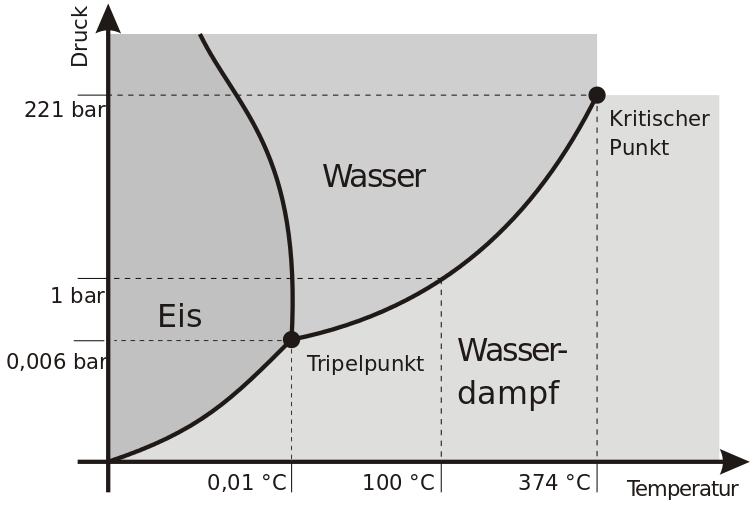
\includegraphics[width=0.7\textwidth]{img/ptwasser2}
			\caption{p-T-Zustandsdiagramm von Wasser \cite{Wikipedia.2019}}
			\label{fig:ptwasser}
		\end{figure}
		\FloatBarrier
		%Ende}
		
		\item \textit{Was sind reduzierte thermodynamische Größen und in welchem Zusammenhang stehen diese zum Korrespondenzprinzip und zu generalisierten Zustandsgleichungen?} 
		
		\textbf{Reduzierte Größen:}\\
		Als reduzierte, thermodynamische Größen bezeichnet man definierte Größen, welche das Verhältnis der jeweiligen thermodynamischen Größe zu ihrem kritischen Wert darstellen \cite{Foth.2008}. 
		\begin{flalign}
			\vartheta &=\frac{T}{T_k}
		\end{flalign}
		\begin{flalign}
		\pi &=\frac{p}{p_k}
		\end{flalign}
			\begin{flalign}
		\varphi &=\frac{V}{V_k}
		\end{flalign}
		\newpage
		Das Korrespondenzprinzip beschreibt dabei ein bestimmtes Verhältnis zu einer alten Theorie, wie der ursprünglichen \textsc{Van-der-Waals}-Gleichung und einer neueren Theorie, wie zum Beispiel der angepassten \textsc{Van-der-Waals}-Gleichung mit reduzierten, thermodynamischen Größen (siehe \eqref{gl1},\eqref{gl2}).
		\begin{flalign}
		\label{gl1}
		\left(p+\frac{a}{{V_m}^2}\right)*\left(V_m-b\right)&= R*T
		\end{flalign}
		\begin{flalign}
			\label{gl2}
			\left(\pi+\frac{3}{\varphi^2}\right)\left(3*\varphi-1\right) &= 8*\vartheta
		\end{flalign}
		Mit der neueren Theorie wird kein Widerspruch zur alten Theorie ausgedrückt. Jedoch beschreibt die ältere Theorie dabei lediglich einen eingeschränkteren Gültigkeitsbereich, als es die neue, erweiterte Theorie kann.
		
		\item \textit{Warum kann vom Manometerstand einer Flüssiggas-Druckflasche nicht auf ihren Füllstand geschlossen werden? Wie wird hier typischerweise der Füllstand überprüft?}
		
		Allein über den Druck lässt sich die Füllmenge des Gases in der Druckflasche nicht bestimmen, da der Druck des Gases eine Funktion der Temperatur darstellt. Den Füllstand Flasche sollte man aus diesem Grund über die Masse bestimmen. Dafür wird jedoch auch das Leergewicht der Gasflasche benötigt.
		 
		\item \textit{Übertragen Sie ihre experimentell aufgenommene Druck-, Temperatur-, Volumen- und Höhenwerte in ein Datenauswerte-Programm, z.B. Excel. Führen Sie die Druckkorrektur aus und bestimmen Sie die Stoffmenge n gemäß Abschnitt 5.2.}
		
		siehe Abschnitt \ref{sec:ergebnisse}
	
		\item \textit{Erstellen und beschreiben Sie ein (pV/R*T)-p-Zustandsdiagramm und ein p-Vm-Zustandsdiagramm mit allen von Ihnen experimentell aufgenommenen Isothermen.}
			\begin{figure}[h!]
				\begin{center}
					\resizebox{0.4\textwidth}{!}{
						\begin{tikzpicture}[trim axis left, trim axis right]
						\begin{axis}[
						axis lines = left,
						width = 15cm,
						height = 11cm,
						xmin = 1000,
						xmax = 5000,
						ymin = 0,
						ymax = 4.0e-6,
						%	ytick = {-4.5,-4,...,-1},
						%	xtick = {-10,-9,...,20},
						ylabel={Stoffmenge in \si{\kilo \mol}},
						%y label style={at={(0,0.5)}},
						xlabel={Druck in \si{\kilo \pascal}},
						legend style={at={(0.75,0.6)},anchor=west},
						%	y dir = reverse,
						]
							\addplot [color=black, mark=*] coordinates{(1715.593552,2.72274396362054E-06) (1783.392808,2.68882795533436E-06) (1863.058648,2.66110146754721E-06) (1929.457656,2.60283462993869E-06) (2020.123496,2.56484016186231E-06) (2108.789336,2.51007592756214E-06) (2194.588592,2.43805532153746E-06) (2296.121016,2.3686480161337E-06) (2406.053688,2.29112594210156E-06) (2513.31928,2.19382888776975E-06) (2619.251952,2.07845046782657E-06) (2676.65096,1.91159838296396E-06) (2680.717048,1.70177980725278E-06) (2681.98264,1.48976032946659E-06) (2683.64848,1.27773055993616E-06) (2686.180904,1.06578024163015E-06) (2698.113576,8.56411758327314E-07) (2705.31308,7.51359842018043E-07) (2721.779416,6.47942672661136E-07) (2735.97892,5.42769154175439E-07) (3482.712088,5.52726098997967E-07) (4850.045008,6.73513368550911E-07) };
							
								\addplot [color=brown, mark=*] coordinates{(1809.726968,2.7804213411711E-06) (1884.392808,2.75037934870788E-06) (1965.791816,2.71817608552944E-06) (2049.591072,2.67660140414793E-06) (2147.256912,2.63919543607175E-06) (2242.789336,2.58432602424148E-06) (2345.32176,2.52230748179461E-06) (2460.121016,2.45678630655597E-06) (2585.786856,2.38364474374417E-06) (2717.586112,2.29637895977425E-06) (2859.98512,2.19700645558369E-06) (3001.65096,2.07524921768687E-06) (3146.583632,1.93373441118826E-06) (3285.116056,1.7665108787914E-06) (3358.781896,1.54810571358699E-06) (3365.047488,1.29249467117537E-06) (3368.113576,1.03493786983214E-06) (3375.713328,9.07613949696203E-07) (3385.512584,7.8021311549773E-07) (3416.97892,6.56220612245125E-07) (4690.31184,7.38623530038516E-07) (4910.178424,7.5438809944548E-07) };
						
						\addplot [color=blue, mark=*] coordinates{(1900.726968,2.82986389056993E-06) (1983.259392,2.80510379547671E-06) (2070.791816,2.77475575149913E-06) (2162.32424,2.73643762679967E-06) (2265.256912,2.69807030512243E-06) (2372.789336,2.64951422860374E-06) (2488.455176,2.59342488168714E-06) (2619.254432,2.53476005779796E-06) (2758.65344,2.46430357054391E-06) (2911.719528,2.38428430267054E-06) (3075.251952,2.28926736977025E-06) (3260.784376,2.18464264050977E-06) (3451.183384,2.05529345403943E-06) (3638.715808,1.8961032942985E-06) (3834.381648,1.7126254876717E-06) (3997.31432,1.48783276660308E-06) (4118.113576,1.2262361824908E-06) (4268.646,9.5329476934841E-07) (4772.845504,8.88245877395173E-07)};
						
						
						\addplot [color=red, mark=*] coordinates{(1950.726968,2.86005279815834E-06) (2031.392808,2.82940475063201E-06) (2122.925232,2.80126871402144E-06) (2217.591072,2.76361761870505E-06) (2327.123496,2.7295243980632E-06) (2439.65592,2.68267094332018E-06) (2561.588592,2.62896608204171E-06) (2696.254432,2.56951875046436E-06) (2848.786856,2.50604444984312E-06) (3011.31928,2.42827046060589E-06) (3181.98512,2.33262921860477E-06) (3380.784376,2.23052733054079E-06) (3594.450216,2.10799718602376E-06) (3819.849224,1.96016137793788E-06) (4049.64848,1.78121418170423E-06) (4271.447736,1.56564273857082E-06) (4369.513824,1.44142881083993E-06) (4476.446496,1.31262586068794E-06) (4593.912832,1.17868664165102E-06) (4800.512584,1.05573868155471E-06) };
						
						
						\legend{Messreihe 1: T=\SI{303,15}{\kelvin}, Messreihe 2: T=\SI{313,15}{\kelvin}, Messreihe 3: T=\SI{323,15}{\kelvin}, Messreihe 3: T=\SI{323,15}{\kelvin}, Messreihe 4: T=\SI{328,15}{\kelvin}}
						\end{axis}
						\end{tikzpicture}
					}
					\caption{Berechnete Stoffmengen in Abhängigkeit vom Druck der Messreihen 1 bis 4 von \ce{SF6}}
					\label{dia:pvrt}
				\end{center}
			\end{figure}
			\FloatBarrier
			
			\newpage
			In Abb. \ref{dia:pvrt} sind die berechneten Stoffmengen über den vorherrschenden Druck aufgetragen. Zu sehen ist, dass die überkritischen Messreihen 3 und 4 einen deutlicher ausgeprägten, linearen Verlauf aufweisen, als die unterkritischen Messreihen 1 und 2. Zudem nähern sich die überkritischen Messreihen deutlich stärker aneinander an, als es die unterkritischen Messreihen in ihrem Verlauf zeigen.\linebreak 
			Grund für diese unterschiedlichen Verläufe der Graphen lässt sich wiederholt über die Phasenübergänge erklären, bei welchen in den Messreihen 1 und 2 isobare Verläufe erkennbar sind (mehr dazu unter Abschnitt \ref{sec:ergebnisse}).
			
	\begin{figure}[h!]
	\begin{center}
		\resizebox{0.4\textwidth}{!}{
			\begin{tikzpicture}[trim axis left, trim axis right]
			\begin{axis}[
			axis lines = left,
			width = 15cm,
			height = 11cm,
			xmin = 0,
			xmax = 1,
			ymin = 1500,
			ymax = 5000,
			%	ytick = {-4.5,-4,...,-1},
			%	xtick = {-10,-9,...,20},
			ylabel={Druck in \si{\kilo \pascal}},
			y label style={at={(-0.05,0.5)}},
			xlabel={molares Volumen in \si{ \liter \per \kilo \mol}},
			legend style={at={(0.75,0.6)},anchor=west},
			%	y dir = reverse,
			]
			\addplot [color=black, mark=*] coordinates{(0.935094018386433,1715.593552) (0.888339317467111,1783.392808) (0.841584616547789,1863.058648) (0.794829915628468,1929.457656) (0.748075214709146,2020.123496) (0.701320513789824,2108.789336) (0.654565812870503,2194.588592) (0.607811111951181,2296.121016) (0.561056411031859,2406.053688) (0.514301710112538,2513.31928) (0.467547009193216,2619.251952) (0.420792308273894,2676.65096) (0.374037607354573,2680.717048) (0.327282906435251,2681.98264) (0.280528205515929,2683.64848) (0.233773504596608,2686.180904) (0.187018803677286,2698.113576) (0.163641453217625,2705.31308) (0.140264102757965,2721.779416) (0.116886752298304,2735.97892) (0.093509401838643,3482.712088) (8.18207266088129E-02,4850.045008) };
			
			\addplot [color=brown, mark=*] coordinates{(0.935094018386433,1809.726968) (0.888339317467111,1884.392808) (0.841584616547789,1965.791816) (0.794829915628468,2049.591072) (0.748075214709146,2147.256912) (0.701320513789824,2242.789336) (0.654565812870503,2345.32176) (0.607811111951181,2460.121016) (0.561056411031859,2585.786856) (0.514301710112538,2717.586112) (0.467547009193216,2859.98512) (0.420792308273894,3001.65096) (0.374037607354573,3146.583632) (0.327282906435251,3285.116056) (0.280528205515929,3358.781896) (0.233773504596608,3365.047488) (0.187018803677286,3368.113576) (0.163641453217626,3375.713328) (0.140264102757965,3385.512584) (0.116886752298304,3416.97892) (9.58471368846093E-02,4690.31184) (9.35094018386433E-02,4910.178424) };
			
			\addplot [color=blue, mark=*] coordinates{(0.935094018386433,1900.726968) (0.888339317467111,1983.259392) (0.841584616547789,2070.791816) (0.794829915628468,2162.32424) (0.748075214709146,2265.256912) (0.701320513789824,2372.789336) (0.654565812870503,2488.455176) (0.607811111951181,2619.254432) (0.561056411031859,2758.65344) (0.514301710112538,2911.719528) (0.467547009193216,3075.251952) (0.420792308273894,3260.784376) (0.374037607354573,3451.183384) (0.327282906435251,3638.715808) (0.280528205515929,3834.381648) (0.233773504596608,3997.31432) (0.187018803677286,4118.113576) (0.140264102757965,4268.646) (0.116886752298304,4772.845504) };
			
			
			\addplot [color=red, mark=*] coordinates{(0.935094018386433,1950.726968) (0.888339317467111,2031.392808) (0.841584616547789,2122.925232) (0.794829915628468,2217.591072) (0.748075214709146,2327.123496) (0.701320513789824,2439.65592) (0.654565812870503,2561.588592) (0.607811111951181,2696.254432) (0.561056411031859,2848.786856) (0.514301710112538,3011.31928) (0.467547009193216,3181.98512) (0.420792308273894,3380.784376) (0.374037607354573,3594.450216) (0.327282906435251,3819.849224) (0.280528205515929,4049.64848) (0.233773504596608,4271.447736) (0.210396154136947,4369.513824) (0.187018803677287,4476.446496) (0.163641453217626,4593.912832) (0.140264102757965,4800.512584) };
			
			\legend{Messreihe 1: T=\SI{303,15}{\kelvin}, Messreihe 2: T=\SI{313,15}{\kelvin}, Messreihe 3: T=\SI{323,15}{\kelvin}, Messreihe 3: T=\SI{323,15}{\kelvin}, Messreihe 4: T=\SI{328,15}{\kelvin}}
			\end{axis}
			\end{tikzpicture}
		}
		\caption{Druck in Abhängigkeit vom molaren Volumen der Messreihen 1 bis 4 von \ce{SF6}}
		\label{dia:pvm}
	\end{center}
\end{figure}
\FloatBarrier
 In Abb. \ref{dia:pvm} ist der Druck in Abhängigkeit vom molaren Volumen aufgetragen. Der Verlauf der Graphen lässt sich hierbei analog auf die schon beschriebene Abb. \ref{dia:isotherme} beziehen. Der Unterschied beider Darstellungen lässt sich auf die Normierung des Volumens auf die berechnete Stoffmenge erklären.

\item \textit{Berechnen Sie den zweiten Virialkoeffizient B mit Hilfe des aus Gleichung 10 erhaltenen Geradenanstiegs b und dem unter Kapitel 5.2 ermittelten Wert der Stoffmenge. Vergleichen Sie den berechneten Virialkoeffizienten B mit Literaturwerten.}
\begin{flalign}
p*V_m&= R*T+B(T)*p\\
\frac{p*V}{R*T}&=n+\frac{B(T)*p*n}{R*T} = a+b*p\\
a+b*p	&=n+\frac{B(T)*p*n}{R*T}\\[1mm] \tag{a=n}
b&=\frac{n}{p}+\frac{B(T)*n}{R*T}-\frac{a}{p}\\
b 				  &= \frac{B(T)*n}{R*T}	\\[1mm]
B(T)			&=\frac{b*R*T}{n}
\end{flalign}

\begin{flalign}
B(T)			&=\frac{b*R*T}{n}\\
B(\SI{323,15}{\kelvin})	&=\frac{\SI{-3,84}{\kmol \per \kilo \pascal}*\SI{8,314}{\joule \per \mole \per \kelvin}*\SI{303,15}{\kelvin}}{\SI{4,28E-06}{\kmol}} =\underline{\SI{ -289	}{\raiseto{3} \centi \meter \per \mole}}	\\		
\end{flalign}
% Table generated by Excel2LaTeX from sheet 'Daten'
\begin{table}[h!]
	\centering
	\caption{experimentell ermittelte Virialkoeffizienten der Messreihen 3 und 4 gegenübergestellt mit Literaturwerte \cite{Lide.1994}}
	%\resizebox{10.5cm}{!}{
		\begin{tabulary}{\textwidth}{C|C|C|C}
			\hline
			\textbf{M3: $T=\SI{323,15}{\kelvin}$}&\textbf{M4: $T=\SI{328,15}{\kelvin}$}&\textbf{Literaturwert \SI{300}{\kelvin}}&\textbf{Literaturwert \SI{350}{\kelvin}}\\
			\hline
			\SI{-289}{\raiseto{3} \centi \meter \per \mole}&	\SI{-274}{\raiseto{3} \centi \meter \per \mole} &	\SI{-275}{\raiseto{3} \centi \meter \per \mole}&	\SI{-190}{\raiseto{3} \centi \meter \per \mole}\\
			\label{tab:Koeffizienten}%
	\end{tabulary}
%}
\end{table}%
\FloatBarrier

Die Virialkoeffizienten der Messreihen 3 und 4 wichen zum Teil ziemlich stark von den Literaturwerten \cite{Lide.1994} ab. Zwar ist die Tendenz, dass mit steigender Temperatur der Wert für den Virialkoeffizient sinkt zu erkennen, jedoch erscheinen die in den Werten selbst vergleichsweise hoch. Grund hierfür könnten Messungenauigkeiten für die Höhe $h$ in der Druckkorrektur sein \mbox{(siehe Abschnitt \ref{sec:fehler})}.

\item \textit{Vergleichen Sie die experimentellen Werte mit theoretisch berechneten Berechnungsergebnissen der CEOS-van-der-Waals und CEOS-PENG-ROBINSONGleichung aus dem PC-Softwareprogramm ZUST.}  
\begin{figure}[h!]
\centering
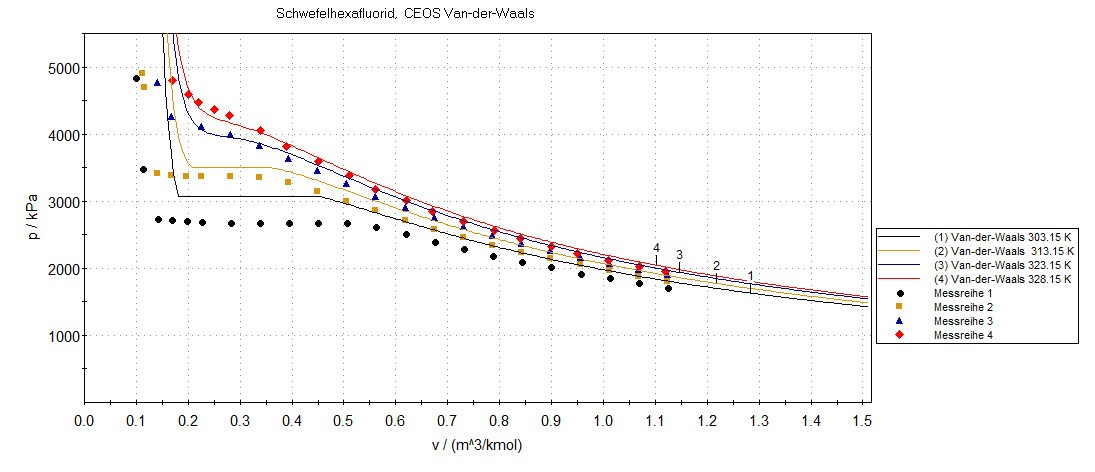
\includegraphics[width=0.85\textwidth]{img/VDW}
\caption{Messdaten mit CEOS-\textsc{Van-der-Waals}-Dampfdruckkurven}
\label{fig:vdW}
\end{figure}
\FloatBarrier
%Ende
\begin{figure}[h!]
	\centering
	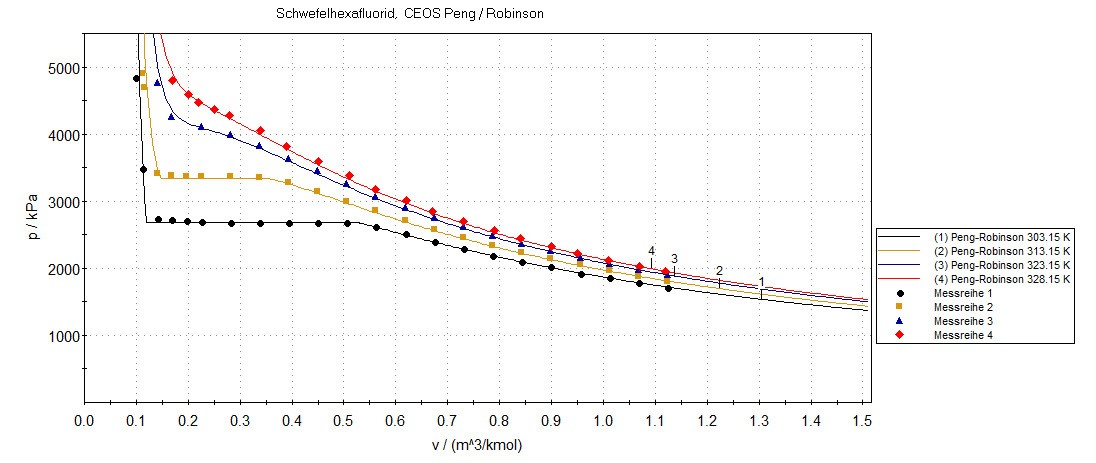
\includegraphics[width=0.85\textwidth]{img/PR}
	\caption{Messdaten mit CEOS-\textsc{Peng-Robinson}-Dampfdruckkurven}
	\label{fig:pr}
\end{figure}
\FloatBarrier
%Ende
In Abb. \ref{fig:vdW} und Abb. \ref{fig:pr} sind aufgenommen Messdaten Druck und molare Volumen gegeneinander aufgetragen. Weiterhin sind in den dargestellten Diagrammen Dampfdruckkurven zwei verschiedener Berechnungsmodell eingezeichnet, welche mit dem Programm \textsc{ZUST} berechnet wurden \cite{zust}. Verwendet wurden die Berechnungsmodelle für die \textsc{Van-der-Waals}-Gleichung (Abb. \ref{fig:vdW}) und der \textsc{Peng-Robinson}-Gleichung (Abb. \ref{fig:pr}).\\
Im Vergleich der beiden Graphen sieht man sofort, dass die \textsc{Peng-Robinson}- Gleichung deutlich besser die aufgenommen Messdaten der Temperaturbereiche erfasst, als es die \textsc{Van-der-Waals}-Gleichung kann. Die \textsc{Van-der-Waals}-Gleichung scheint lediglich im bei den überkritischen Isothermen mit der \textsc{Peng-Robinson}- Gleichung mithalten zu können. Das erklärt sich vermutlich aus dem Zusammenhang heraus, dass sich die \textsc{Van-der-Waals}-Gleichung näher aus dem idealen Gasgesetz ableitet als die \textsc{Peng-Robinson}-Gleichung. So erklärt sich, dass die \textsc{Van-der-Waals}-Gleichung die Messdaten erst unter "`idealeren"' Bedingungen ihren Gültigkeitsbereich ausbildet. Diese "`idealeren"' Bedingungen werden dabei durch höhere Temperaturen , kleinere Drücke und große Volumina ausgedrückt.\\
Müssten man also bestimmte Verläufe von \ce{SF6}-Isothermen voraussagen, so erscheint die \textsc{Peng-Robinson}-Gleichung als qualitativ hochwertiger. 

\end{enumerate}














